\documentclass{article}

\usepackage{graphicx}
\usepackage{tikz}
\usepackage{tikzsymbols}
\usetikzlibrary{calc,patterns,shapes.geometric}
\pagestyle{empty}
\usepackage[margin=0pt]{geometry}
\geometry{papersize={14in,12in}}

\def\centerarc[#1](#2)(#3:#4:#5){\draw[#1] ($(#2)+({#5*cos(#3)},{#5*sin(#3)})$) arc (#3:#4:#5);}

\begin{document}
	\begin{figure}
		\centering
		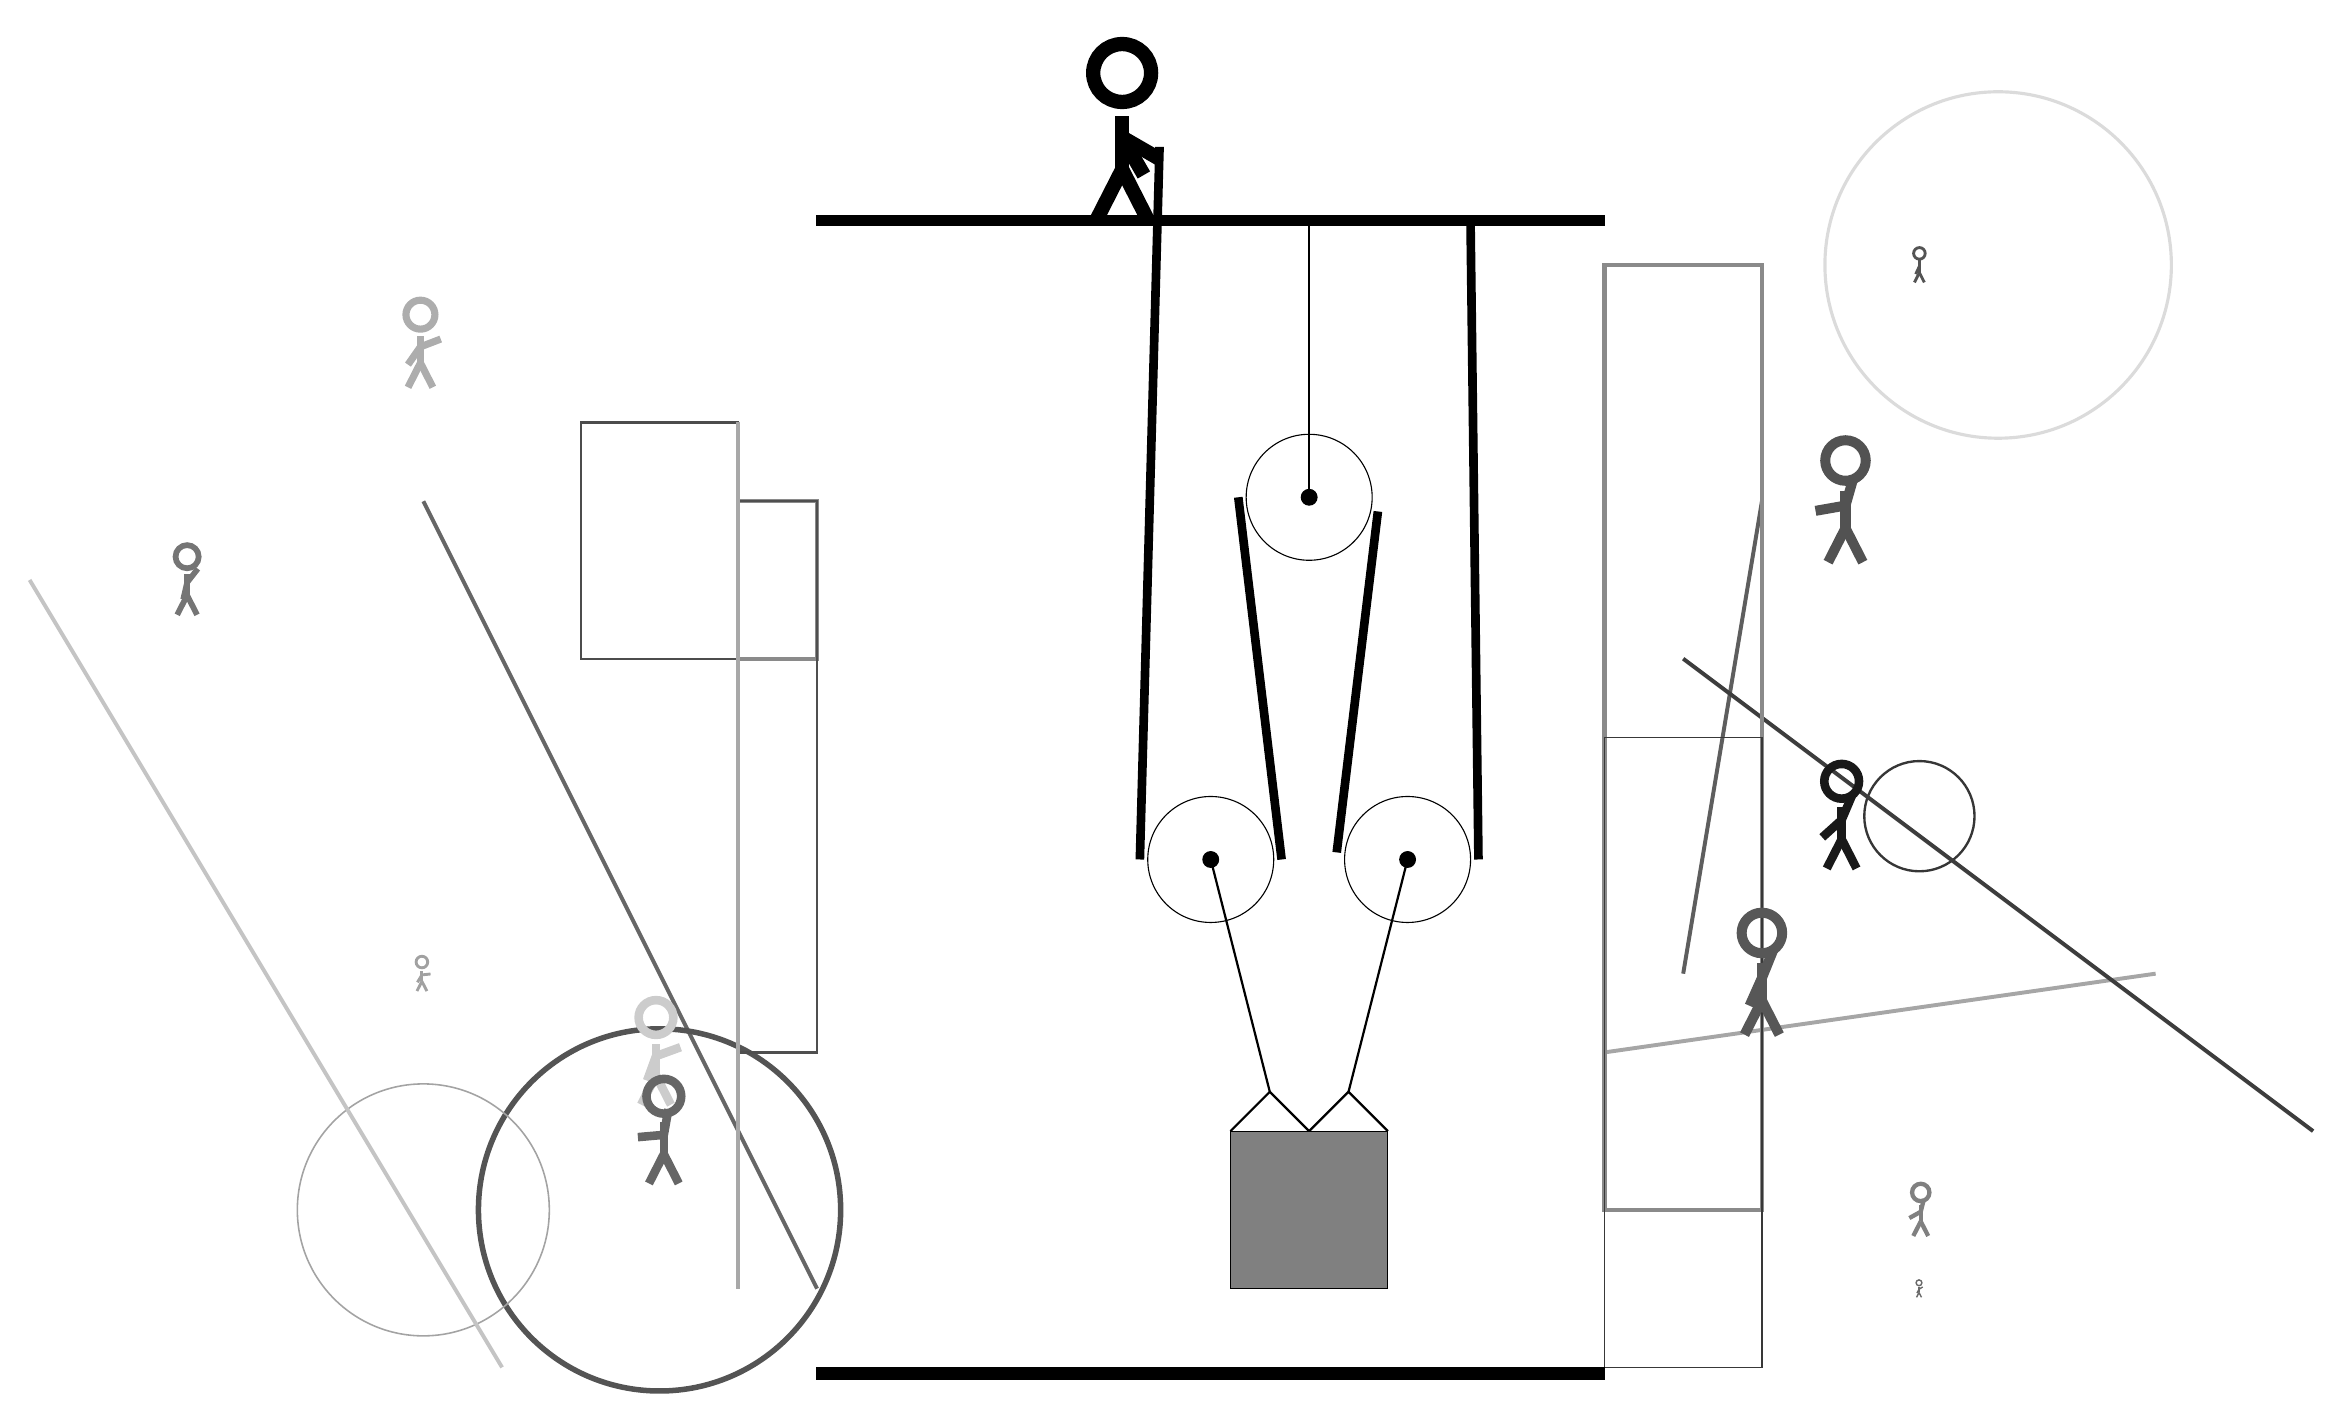
\begin{tikzpicture}
			%%%%% START %%%%%
			
			\draw[fill=black] (-4, 11.5) rectangle (6, 11.625);
			
			\draw (1, 3.45) circle (0.8);
			\draw[fill=black] (1, 3.45) circle (0.1);
			
			\draw (2.25, 8.05) circle (0.8);
			\draw[fill=black] (2.25, 8.05) circle (0.1);
			\draw[thick] (2.25, 8.05) -- (2.25, 11.5);
			
			\node[line width=0.2mm, color=black!54] at (-12, 7) {\Strichmaxerl[4][77][52]};
			
			\draw[line width=0.5mm, color=black!60](-4, -2) -- (-9, 8);
			\node[line width=0.7mm, color=black!68] at (9, 8) {\Strichmaxerl[7][10][74]};
			\draw[line width=0.3mm, color=black!70] (-5, 9) rectangle (-7, 6);
			\draw [line width=0.7mm, color=black!67](-6, -1) circle (2.3);
			\draw [line width=0.3mm, color=black!79](10, 4) circle (0.7);
			\draw[line width=0.5mm, color=black!35](6, 1) -- (13, 2);
			
			\node[line width=0.7mm, color=black!59] at (10, -2) {\Strichmaxerl[1][62][32]};
			\draw[line width=0.5mm, color=black!46] (-4, 6) rectangle (-5, 8);
			\node[line width=0.2mm, color=black!20] at (-6, 1) {\Strichmaxerl[6][70][20]};
			\draw [line width=0.2mm, color=black!36](-9, -1) circle (1.6);
			\draw[line width=0.5mm, color=black!63](8, 8) -- (7, 2);
			\draw [line width=0.4mm, color=black!14](11, 11) circle (2.2);
			
			\node[line width=0.7mm, color=black!37] at (-9, 2) {\Strichmaxerl[2][59][6]};
			\draw[line width=0.5mm, color=black!76](7, 6) -- (15, 0);
			\draw[line width=0.5mm, color=black!60](6, 3) -- (6, 2);
			\draw[line width=0.6mm, color=black!46] (6, 11) rectangle (8, -1);
			\node[line width=0.3mm, color=black!50] at (10, -1) {\Strichmaxerl[3][29][76]};
			\node[line width=0.2mm, color=black!90] at (9, 4) {\Strichmaxerl[6][42][67]};
			\draw[line width=0.2mm, color=black!78] (6, -3) rectangle (8, 5);
			\node[line width=0.5mm, color=black!66] at (8, 2) {\Strichmaxerl[7][66][68]};
			
			\draw[line width=0.3mm, color=black!69] (-4, 1) rectangle (-5, 8);
			
			\node[line width=0.3mm, color=black!67] at (10, 11) {\Strichmaxerl[2][65][90]};
			\node[line width=0.5mm, color=black!60] at (-6, 0) {\Strichmaxerl[6][5][80]};
			\draw[line width=0.5mm, color=black!34](-5, -2) -- (-5, 9);
			
			\draw[line width=0.5mm, color=black!23](-8, -3) -- (-14, 7);
			
			\node[line width=0.3mm, color=black!32] at (-9, 10) {\Strichmaxerl[5][55][21]};
			
			\draw (3.5, 3.45) circle (0.8);
			\draw[fill=black] (3.5, 3.45) circle (0.1);
			
			\draw[thick] (3.5, 3.45) -- (2.75, 0.5);
			\draw[thick] (1, 3.45) -- (1.75, 0.5);
			\draw[thick]  (1.25, 0) -- (1.75, 0.5) -- (2.25, 0);
			\draw[thick]  (2.25, 0) -- (2.75, 0.5) -- (3.25, 0);
			\draw[fill=black!50] (1.25, 0) rectangle (3.25, -2);
			
			\draw[line width=1.1mm] (0.35, 12.5) --  (0.1, 3.45);
			\centerarc[line width=1.1mm](1, 3.45)(180:360:0.9);
			\draw[line width=1.1mm] (1.9, 3.45) -- (1.35, 8.05);
			\centerarc[line width=1.1mm](2.25, 8.05)(-20:180:0.9);
			\draw[line width=1.1mm](3.123, 7.87) -- (2.6, 3.54);
			\centerarc[line width=1.1mm](3.5, 3.45)(160:360:0.9);
			\draw[line width=1.1mm](4.4, 3.45) -- (4.3, 11.5);
			
			\node at (-0.07, 12.7) {\Strichmaxerl[10][120][-30]};
			
			\draw[fill=black] (-4, -3) rectangle (6, -3.15);
			
			%%%%% END %%%%%
		\end{tikzpicture}
	\end{figure}	
\end{document}